% Mohamed bin Zayed University of Artificial Intelligence (MBZUAI) Thesis Template for LaTeX 

% uOttawa (unofficial) Thesis Template for LaTeX

% Edited by Wail Gueaieb based on the uWaterloo’s Template
% The updated version of this template has been edited by Moayad Aloqaily and Mohsen Guizani.


% DON'T USE THIS TEMPLATE IF YOU DON'T KNOW WHAT YOU'RE DOING!
% Remember, it comes WITH NO WARRANTY!

% Please read the "00readme.txt" file first.
% Here is how to use this template:
%
% DON'T FORGET TO ADD YOUR OWN NAME AND TITLE in the "hyperref" package
% configuration in the "thesis-preample.tex" file. THIS INFORMATION GETS 
% EMBEDDED IN THE PDF FINAL PDF DOCUMENT.
% You can view the information if you view Properties of the PDF document.

% The template is based on the standard "book" document class which provides 
% all necessary sectioning structures and allows multi-part theses.




% N.B. The "pdftex" program allows graphics in the following formats to be
% included with the "\includegraphics" command: PNG, PDF, JPEG, TIFF
% Tip 1: Generate your figures and photos in the size you want them to appear
% in your thesis, rather than scaling them with \includegraphics options.
% Tip 2: Any drawings you do should be in scalable vector graphic formats:
% SVG, PNG, WMF, EPS and then converted to PNG or PDF, so they are scalable in
% the final PDF as well.
% Tip 3: Photographs should be cropped and compressed so as not to be too large.

% To create a PDF output that is optimized for double-sided printing: 
%
% 1) comment-out the \documentclass statement in the preamble below, and
% un-comment the second \documentclass line.
%
% 2) change the value assigned below to the boolean variable
% "PrintVersion" from "false" to "true".

% --------------------- Start of Document Preamble -----------------------

% Specify the document class, default style attributes, and page dimensions
% For hyperlinked PDF, suitable for viewing on a computer, use this:
\documentclass[letterpaper,12pt,titlepage,oneside,final]{book}
\usepackage{graphicx}
\graphicspath{ {./images/} }
% For PDF, suitable for double-sided printing, change the PrintVersion variable below
% to "true" and use this \documentclass line instead of the one above:
% \documentclass[letterpaper,12pt,titlepage,openright,twoside,final]{book}


% This package allows if-then-else control structures.
\usepackage{ifthen}
\newboolean{PrintVersion}
\setboolean{PrintVersion}{false} 
% \setboolean{PrintVersion}{true} 
% CHANGE THIS VALUE TO "true" as necessary, to improve printed results 
% for hard copies by overriding some options of the hyperref package.


% Load your needed packages and other commands of yours.
% Load your needed packages and other commands of yours here:
%\usepackage{} % ... note that old .sty files can be included here

















%--------------------------------------------------------------------------
% Do NOT edit the rest of the preample UNLESS YOU KNOW WHAT YOU'RE DOING!
%--------------------------------------------------------------------------

\ifthenelse{\boolean{PrintVersion}}{
\usepackage[top=1in,bottom=1in,left=0.75in,right=1.25in]{geometry}   % For twoside document
}{
\usepackage[top=1in,bottom=1in,left=0.75in,right=1.25in]{geometry}   % For oneside document
}

\usepackage{amsmath,amssymb,amstext} % Lots of math symbols and environments
\usepackage{graphicx} % For including graphics 

%\usepackage{nomentbl} 
%\makenomenclature 

\usepackage{ifpdf}

\newcommand{\href}[1]{#1} % does nothing, but defines the command so the
    % print-optimized version will ignore \href tags (redefined by hyperref pkg).
%\newcommand{\texorpdfstring}[2]{#1} % does nothing, but defines the command
% Anything defined here may be redefined by packages added below...


% Hyperlinks make it very easy to navigate an electronic document.
% In addition, this is where you should specify the thesis title
% and author as they appear in the properties of the PDF document.
% Use the "hyperref" package 
% N.B. HYPERREF MUST BE THE LAST PACKAGE LOADED; ADD ADDITIONAL PKGS ABOVE
\usepackage[\ifpdf pdftex,\fi letterpaper=true,pagebackref=false]{hyperref} % with basic options
		% N.B. pagebackref=true provides links back from the References to the body text. This can cause trouble for printing.
\ifthenelse{\boolean{PrintVersion}}{   % for improved print quality, change some hyperref options
\hypersetup{	% override some previously defined hyperref options
%    colorlinks,%
    citecolor=black,%
    filecolor=black,%
    linkcolor=black,%
    urlcolor=black}
}{} % end of ifthenelse (no else)



% This is where thesis margins and spaces are set.
% Setting up the page margins...
% A minimum of 1 inch (72pt) margin at the
% top, bottom, and outside page edges and a 1.125 in. (81pt) gutter
% margin (on binding side). While this is not an issue for electronic
% viewing, a PDF may be printed, and so we have the same page layout for
% both printed and electronic versions, we leave the gutter margin in.
% Set margins:
\setlength{\marginparwidth}{0pt} % width of margin notes
% N.B. If margin notes are used, you must adjust \textwidth, \marginparwidth
% and \marginparsep so that the space left between the margin notes and page
% edge is less than 15 mm (0.6 in.)
\setlength{\marginparsep}{0pt} % width of space between body text and margin notes
\setlength{\evensidemargin}{0.125in} % Adds 1/8 in. to binding side of all 
% even-numbered pages when the "twoside" printing option is selected
\setlength{\oddsidemargin}{0.125in} % Adds 1/8 in. to the left of all pages
% when "oneside" printing is selected, and to the left of all odd-numbered
% pages when "twoside" printing is selected
\setlength{\textwidth}{6.375in} % assuming US letter paper (8.5 in. x 11 in.) and 
% side margins as above
\raggedbottom

% The following statement specifies the amount of space between
% paragraphs. Other reasonable specifications are \bigskipamount and \smallskipamount.
\setlength{\parskip}{\medskipamount}

% The following statement controls the line spacing.  The default
% spacing corresponds to good typographic conventions and only slight
% changes (e.g., perhaps "1.2"), if any, should be made.
\renewcommand{\baselinestretch}{1} % this is the default line space setting

% By default, each chapter will start on a recto (right-hand side)
% page.  We also force each section of the front pages to start on 
% a recto page by inserting \cleardoublepage commands.
% In many cases, this will require that the verso page be
% blank and, while it should be counted, a page number should not be
% printed.  The following statements ensure a page number is not
% printed on an otherwise blank verso page.
\let\origdoublepage\cleardoublepage
\newcommand{\clearemptydoublepage}{%
  \clearpage{\pagestyle{empty}\origdoublepage}}
\let\cleardoublepage\clearemptydoublepage



%======================================================================
%   L O G I C A L    D O C U M E N T -- the content of your thesis
%======================================================================
\begin{document}

% For a large document, it is a good idea to divide your thesis
% into several files, each one containing one chapter.
% To illustrate this idea, the "front pages" (i.e., title page,
% declaration, borrowers' page, abstract, acknowledgements,
% dedication, table of contents, list of tables, list of figures,
% nomenclature).
%----------------------------------------------------------------------
% FRONT MATERIAL
%----------------------------------------------------------------------
%
% C O V E R  P A G E
% ------------------
\newcommand{\thesisauthor}{Shivam Grover}
\newcommand{\thesistitlecoverpage}{%
  Transmission Dynamics of Monkeypox Virus
}
\newcommand{\degree}{B.Sc.} % possible values are:
                            % M.A. / M.A.Sc. / M.Sc. / MCS / Ph.D.
\newcommand{\nameofprogram}{Applied Mathematics and Computer Science}
\newcommand{\academicunit}{Departement of Mathematics}
\newcommand{\faculty}{Faculty of Science}
\newcommand{\graduationyear}{2022}
%
% T I T L E   P A G E
% -------------------
% Last updated May 24, 2011, by Stephen Carr, IST-Client Services
% The title page is counted as page `i' but we need to suppress the
% page number.  We also don't want any headers or footers.
\pagestyle{empty}
\pagenumbering{roman}

% The contents of the title page are specified in the "titlepage"
% environment.
\begin{titlepage}
        \begin{center}
        \vspace*{1.0cm}

        \Huge
        {\bf \thesistitlecoverpage }

        \vspace*{1.0cm}

        \normalsize
        by \\

        \vspace*{1.0cm}

        \Large
        \thesisauthor \\
        Yuan Yuan \\

        \vspace*{3.0cm}

        \normalsize
        Paper submitted to the\\
        Department of Mathematics\\
        %In partial fulfillment of the requirements\\
        for the Summer Undergraduate Research Apprenticeship (SURA) %\degree~degree in\\
        %\nameofprogram\\

        \vspace*{2.0cm}

        \academicunit\\
        %\faculty\\
        Memorial University of Newfoundland (MUN)\\

        \vspace*{1.0cm}

        \copyright~\thesisauthor, NL, CANADA \graduationyear\\
        \end{center}
\end{titlepage}

% The rest of the front pages should contain no headers and be numbered using Roman numerals starting with `ii'
\pagestyle{plain}
\setcounter{page}{2}

\cleardoublepage % Ends the current page and causes all figures and tables that have so far appeared in the input to be printed.
% In a two-sided printing style, it also makes the next page a right-hand (odd-numbered) page, producing a blank page if necessary.

%
%
% R E S T  O F  F R O N T  P A G E S
% ----------------------------------
%\cleardoublepage % Ends the current page and causes all figures and tables that have so far appeared in the input to be printed.
% In a two-sided printing style, it also makes the next page a right-hand (odd-numbered) page, producing a blank page if necessary.

 
% E X A M I N I N G   C O M M I T T E E (Required for Ph.D. theses only)
% Remove or comment out the lines below to remove this page
\begin{center}\textbf{Examining Committee Membership}\end{center}
  \noindent
The following served on the Examining Committee for this thesis. The decision of the Examining Committee is by majority vote.
  \bigskip
  
  \noindent
\begin{tabbing}
Internal-External Member: \=  \kill % using longest text to define tab length
External Examiner: \>  Name X! \\ 
\> Professor, Dept. of , University of \\
\end{tabbing} 
  \bigskip
  
  \noindent
\begin{tabbing}
Internal-External Member: \=  \kill % using longest text to define tab length
Supervisor(s): \> Name 1!\\
\> Professor, Dept. of ML, \\Mohamed bin Zayed University of Artificial Intelligence (MBZUAI) \\
\> Name 2! \\
\> Professor , Dept. of CV, \\Mohamed bin Zayed University of Artificial Intelligence (MBZUAI) \\
\end{tabbing}
  \bigskip
  
  \noindent
  \begin{tabbing}
Internal-External Member: \=  \kill % using longest text to define tab length
Internal Member: \> Name Y! \\
\> Professor, Dept. of , University of  \\
\end{tabbing}
  \bigskip
  
  \noindent
\begin{tabbing}
Internal-External Member: \=  \kill % using longest text to define tab length
Internal-External Member: \> Name Z! \\
\> Professor, Dept. of , University of  \\
\end{tabbing}
  \bigskip
  
  \noindent
\begin{tabbing}
Internal-External Member: \=  \kill % using longest text to define tab length
Other Member(s): \> Name R! \\
\> Professor, Dept. of , University of \\
\end{tabbing}

\cleardoublepage
%% D E C L A R A T I O N   P A G E
% -------------------------------

\begin{center}\textbf{Author's Declaration}\end{center}

  \noindent
I hereby declare that I am the sole author of this thesis. This is a true copy of the thesis, including any required final revisions, as accepted by my examiners.

  \bigskip
  
  \noindent
I understand that my thesis may be made electronically available to the public.

\cleardoublepage
%\newpage


% Edit the following 3 files with your abstract, acknowledgements, 
% and dedication.
% A B S T R A C T
% ---------------

\begin{center}\textbf{Abstract}\end{center}

The abstract should not exceed 500 words or 2 pages. The abstract should explain the domain of the thesis, identify topic area, include the hypothesis or problem statement, provide a general overview of the methodology, and identify research benefits and key findings and/or contributions.



\cleardoublepage
%\newpage

%% A C K N O W L E D G E M E N T S
% -------------------------------

\begin{center}\textbf{Acknowledgements}\end{center}

I would like to thank ...


\cleardoublepage
%\newpage
%% D E D I C A T I O N
% -------------------

\begin{center}\textbf{Dedication}\end{center}

This is dedicated to ...


\cleardoublepage
%\newpage


% No need to edit this file.
% T A B L E   O F   C O N T E N T S
% ---------------------------------
\renewcommand\contentsname{Table of Contents}
\tableofcontents
\cleardoublepage
\phantomsection
%\newpage

% L I S T   O F   T A B L E S
% ---------------------------
%\addcontentsline{toc}{chapter}{List of Tables}
%\listoftables
%\cleardoublepage
%\phantomsection		% allows hyperref to link to the correct page
%\newpage

% L I S T   O F   F I G U R E S
% -----------------------------
%\addcontentsline{toc}{chapter}{List of Figures}
%\listoffigures
%\cleardoublepage
%\phantomsection		% allows hyperref to link to the correct page
%\newpage


%% L I S T   O F   S Y M B O L S
% -----------------------------
% To include a Nomenclature section


%\addcontentsline{toc}{chapter}{\textbf{List of Acronyms}}
%\cleardoublepage
%\phantomsection	


%\renewcommand{\nomname}{List of Acronyms}
%\renewcommand{\nomAname}{\textbf{\large Abbreviations}}
%\textbf{List of Acronyms}



\chapter*{List of Abbreviations}
%\addcontentsline{toc}{chapter}{List of Acronyms}
\begin{longtable}{cp{0.8\textwidth}}


AI      &Artificial Intelligence.\\

\end{longtable}


\renewcommand{\nomGname}{\textbf{\large Mathematical Symbols}}
%\textbf{List of Symbols}

\renewcommand{\nomXname}{\textbf{\large Superscripts}}
\renewcommand{\nomZname}{\textbf{\large Subscripts}}

%\printnomenclature
%\cleardoublepage
%\phantomsection % allows hyperref to link to the correct page
% \newpage

%
% No need to edit this file. But you may want to comment the whole line if you
% don't have or want a Nomenclature section.
%% L I S T   O F   S Y M B O L S
% -----------------------------
% To include a Nomenclature section
\addcontentsline{toc}{chapter}{\textbf{Nomenclature}}

\renewcommand{\nomname}{Nomenclature}
\renewcommand{\nomAname}{\textbf{\large Abbreviations}}
\renewcommand{\nomGname}{\textbf{\large Mathematical Symbols}}
\renewcommand{\nomXname}{\textbf{\large Superscripts}}
\renewcommand{\nomZname}{\textbf{\large Subscripts}}

\printnomenclature
\cleardoublepage
\phantomsection % allows hyperref to link to the correct page
% \newpage






%%% Local Variables: 
%%% mode: latex
%%% TeX-master: "../uottawa-thesis"
%%% End:   


% Change page numbering back to Arabic numerals
\pagenumbering{arabic}

%----------------------------------------------------------------------
% MAIN BODY
%---------------------------------------------------------------------- 
% Chapters 
% Include your "sub" source files here (must have extension .tex)
%======================================================================
\chapter{Introduction}
%======================================================================
Monkeypox is a viral zoonosis (a virus transmitted to humans from animals) with symptoms very similar to those seen in the past in smallpox patients, although it is clinically less severe. It is caused by the monkeypox virus which belongs to the Orthopoxvirus genus of the Poxviridae family. The name monkeypox originates from the initial discovery of the virus in monkeys in Statens Serum Institute, Copenhagen Denmark, in 1958. The first human case was identified in a young child in the Democratic Republic of the Congo in 1970.

%----------------------------------------------------------------------
\section{Background}
%----------------------------------------------------------------------
Monkeypox is commonly found in central and west Africa where there are tropical rainforests and where animals that may carry the virus typically live. People with monkeypox are occasionally identified in other countries outside of central and west Africa, following travel from regions where monkeypox is endemic.
Monkeypox virus is transmitted from one person to another by close contact with lesions, body fluids, respiratory droplets and contaminated materials such as bedding. The incubation period of monkeypox is usually from 6 to 13 days but can range from 5 to 21 days.
Various animal species have been identified as susceptible to the monkeypox virus. Uncertainty remains on the natural history of the monkeypox virus and further studies are needed to identify the reservoir(s) and how virus circulation is maintained in nature. Eating inadequately cooked meat and other animal products of infected animals is a possible risk factor.
Monkeypox is usually self-limiting but there is likely to be little immunity to monkeypox among people living in non-endemic countries since the virus has not previously been identified in those populations. There are two variants of the monkeypox virus: the West African variant and the Congo Basin (Central African) variant. The Congo Basin variant appears to cause severe disease more frequently with a case fatality ratio (CFR) previously reported of up to around 10\%. Currently, the Democratic Republic of the Congo is reporting a CFR among suspected cases of around 3\%. The West African clade has in the past been associated with an overall lower CFR of around 1\% in a generally younger population in the African setting. Since 2017, the few deaths of persons with monkeypox in West Africa have been associated with young age or an untreated HIV infection.

\section{Symptoms}

Symptoms of monkeypox typically include a fever, intense headache, muscle aches, back pain, low energy, swollen lymph nodes, and a skin rash or lesions. The rash usually begins within one to three days of the start of a fever. Lesions can be flat or slightly raised, filled with clear or yellowish fluid, and can then crust, dry up and fall off. The number of lesions on one person can range from a few to several thousand. Symptoms typically last between 2 to 4 weeks and go away on their own without treatment.

\section{OutBreak in Endemic and Non-Endemic Countries}
Since 13 May 2022, monkeypox has been appearing in 23 Member States that are not endemic to the monkeypox virus, across four WHO regions. Epidemiological investigations are ongoing. The vast majority of reported cases so far have no established travel links to an endemic area and have presented through primary care or sexual health services. The identification of confirmed and suspected cases of monkeypox with no direct travel links to an endemic area is atypical. Early epidemiology of initial cases notified to WHO by countries shows that cases have been mainly reported amongst men who have sex with men (MSM). One case of monkeypox in a non-endemic country is considered an outbreak. The sudden appearance of monkeypox simultaneously in several non-endemic countries suggests that there may have been undetected transmission for some time as well as recent amplifying events.
As of 26 May, a cumulative total of 257 laboratory-confirmed cases and around 120 suspected cases have been reported to WHO. No deaths have been reported.
The situation is evolving rapidly and WHO expects that there will be more cases identified as surveillance expands in non-endemic countries, as well as in countries known to be endemic who have not recently been reporting cases.

\section{Vaccinations}
There are several vaccines available for prevention of smallpox that also provide some protection against monkeypox. A newer vaccine that was developed for smallpox (MVA-BN, also known as Imvamune, Imvanex or Jynneos) was approved in 2019 for use in preventing monkeypox and is not yet widely available. Vaccinia is also known to deliver long-lasting immunity against
monkeypox, with 85\% efficacy.

% Some LaTeX commands I define for my own nomenclature.
% If you have to, it's better to change nomenclature once here than in a 
% million places throughout your thesis!
\newcommand{\package}[1]{\textbf{#1}} % package names in bold text
\newcommand{\cmmd}[1]{\textbackslash\texttt{#1}} % command name in tt font 


%======================================================================
\chapter{Model Description}
%======================================================================

The model is composed of human population given by $N_{h}$ and
reservoir population given by $N_{r}$. We divide the human population ($N_{h}$) in $5$ categories namely, Susceptibles ($S_{h}$), Vaccinated ($V_{h}$), Exposed ($E_{h}$), Infected ($I_{h}$) and Recovered ($R_{h}$) whereas the reservoir population ($N_{r}$) is divided among Susceptibles ($S_{r}$), Infected($I_{r}$) and Recovered ($R_{r}$), such that
\[N_{h} = S_{h} + V_{h} + E_{h} + I_{h} + R_{h}\]
\[N_{r} = S_{r} + I_{r} + R_{r}\]

\begin{figure}[h]
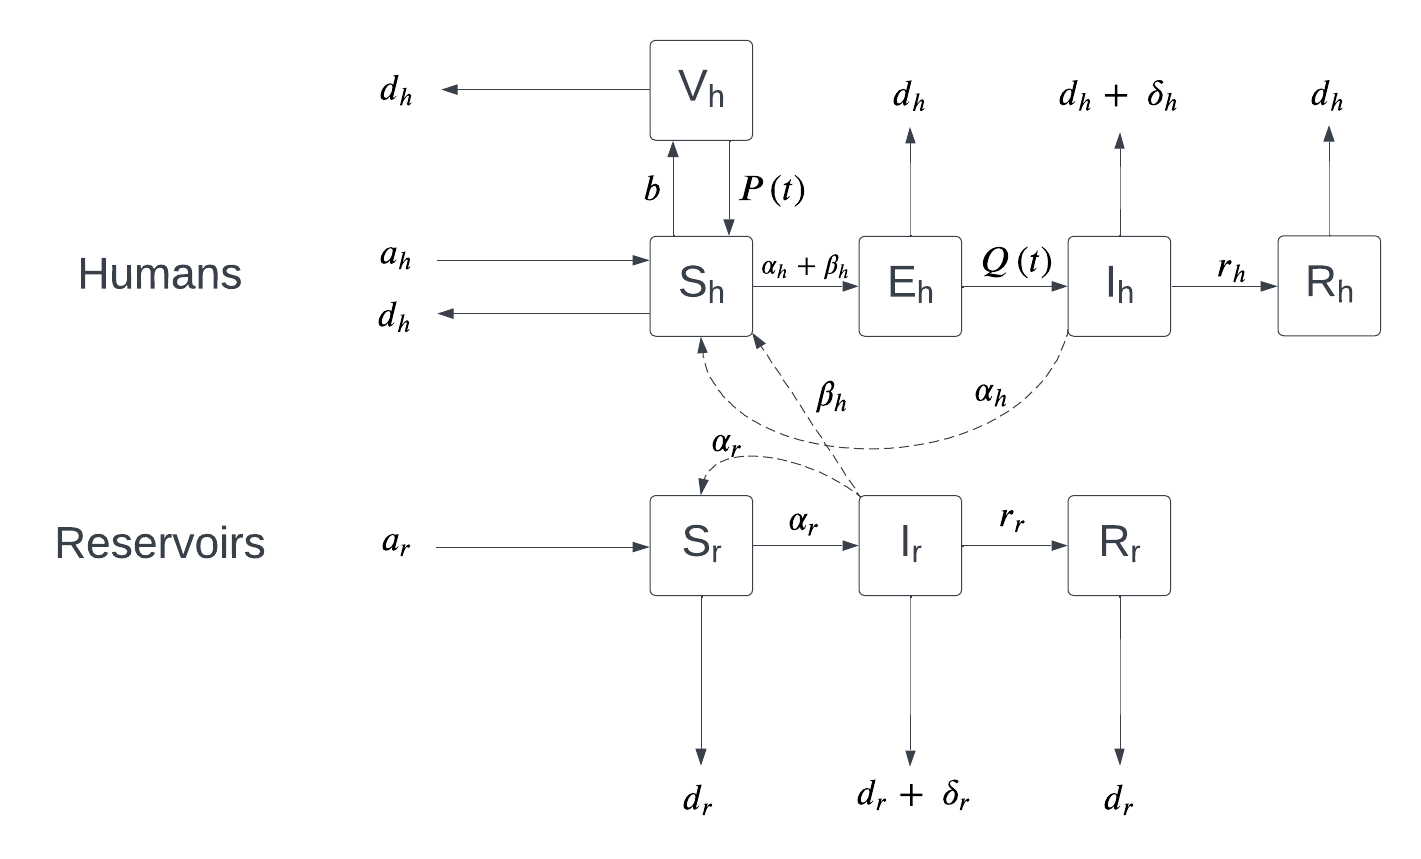
\includegraphics[width=\textwidth]{flow-diagram}
\caption{Model Flow Diagram}
\centering
\end{figure}
We assume that $a_{h}$ and $a_{r}$ is the constant birth rate of susceptible humans and reservoirs respectively and susceptibles are vaccinated at a constant rate $b$. $\alpha_{r}$, $\alpha_{h}$ and $\beta_{h}$ are the infection rates from reservoir to reservoir, reservoir to human and from human to human respectively.
To allow for a general latent period, we further assume that $P(t)$ is the probability of individuals remaining in the vaccinated class $t$ units after being vaccinated and $Q(t)$ is the probability of individuals remaining in the exposed class $t$ units after being exposed to the monkeypox virus. $r_{h}$ and $r_{r}$ are the recovery rates of the humans and the reservoirs respectively from the infection. Lastly, we consider that $d_{h}$ and $\delta_{h}$ is the natural and infection related death rate of humans whereas $d_{r}$ and $\delta_{r}$ is the natural and infection-related death rate of reservoirs.
According to the natural progression of the disease, we assume $P(t)$ and $Q(t)$ non-negative, non-increasing and piecewise continuous with 
\begin{center}
$P(0^{+}) = Q(0^{+}) = 1$ and $P(\infty) = Q(\infty) = 0$
\end{center}

The number of individuals who become exposed at some time $\mu \in (0,t)$ and are still in the exposed class at time $t$ is given by
\begin{equation}
E_{h}(t) = \int_{0}^{t} (\alpha_{h}S_{h}(\mu)I_{h}(\mu) +\beta_{h}S_{h}(\mu)I_{r}(\mu)) e^{-d_{h}(t-\mu)}Q(t-\mu) \,d\mu \label{exposed}
\end{equation}


and the number of individuals who get vaccinated at some time $\mu \in (0,t)$ and are still in the vaccinated class at time $t$ is given by
\begin{equation}
V_{h}(t) = \int_{0}^{t} bS_{h}(\mu)e^{-d_{h}(t-\mu)}P(t-\mu) \,d\mu \label{vaccinated}
\end{equation}


%Now, substituting $v = t-\mu$, we get

%\[E_{h}(t) = \int_{0}^{t} (\beta_{h}S_{h}(t-v)I_{h}(t-v) + \alpha_{h}S_{h}(t-v)I_{r}(t-v)) e^{-d_{h}v}Q(v) \,dv\]

%\[V_{h}(t) = \int_{0}^{t} bS_{h}(t-v)e^{-d_{h}(v)}P(v) \,dv\]
The general model is represented as follows
\begin{flalign} 
S_{h}'(t) &= a_{h}-d_{h}S_{h}(t)-bS_{h}(t)-(\alpha_{h}S_{h}(t)I_{h}(t)+\beta_{h}S_{h}(t)I_{r}(t))-\int_{0}^{t} bS_{h}(\mu)e^{-d_{h}(t-\mu)}P'(t-\mu) \,d\mu  \label{meq1}\\
%-------------------------------------------------------------
V_{h}'(t) &= bS_{h}(t)-d_{h}V_{h}(t)+\int_{0}^{t} bS_{h}(\mu)e^{-d_{h}(t-\mu)}P'(t-\mu) \,d\mu  \label{meq2}\\
%-------------------------------------------------------------
E_{h}'(t) &= \alpha_{h}S_{h}(t)I_{h}(t)+\beta_{h}S_{h}(t)I_{r}(t))-d_{h}E_{h}(t)+\int_{0}^{t} (\alpha_{h}S_{h}(\mu)I_{h}(\mu)+\beta_{h}S_{h}(\mu)I_{r}(\mu))e^{-d_{h}(t-\mu)}Q'(t-\mu) \,d\mu  \label{meq3}\\
%-------------------------------------------------------------
I_{h}'(t) &= -\int_{0}^{t} (\alpha_{h}S_{h}(\mu)I_{h}(\mu)+\beta_{h}S_{h}(\mu)I_{r}(\mu))e^{-d_{h}(t-\mu)}Q'(t-\mu) \,d\mu -d_{h}I_{h}(t) -\delta_{h}I_{h}(t) -r_{h}I_{h}(t)  \label{meq4}\\
%-------------------------------------------------------------
R_{h}'(t) &= r_{h}I_{h}(t) -d_{h}R_{h}(t) \label{meq5}\\ 
%-------------------------------------------------------------
S_{r}'(t) &= a_{r}-d_{r}S_{r}(t)-\alpha_{r}S_{r}(t)I_{r}(t)  \label{meq6}\\
%-------------------------------------------------------------
I_{r}'(t) &= \alpha_{r}S_{r}(t)I_{r}(t) -d_{r}I_{r}(t) -\delta_{r}I_{r}(t)- r_{r}I_{r}(t)  \label{meq7}\\
%-------------------------------------------------------------
R_{r}'(t) &= r_{r}I_{r}(t) -d_{r}R_{r}(t)  \label{meq8}
%-------------------------------------------------------------
\end{flalign}

To obtain more specific models, we have discussed four cases with different values for the functions $P(t)$ and $Q(t)$.

% CASE 1
Case \rom{1} [$P(t)=e^{-\omega_{1} t}, Q(t)=e^{-\omega_{2} t}$]

Equation \ref{exposed} becomes
\[E_{h}(t) = \int_{0}^{t} (\alpha_{h}S_{h}(\mu)I_{h}(\mu) + \beta_{h}S_{h}(\mu)I_{r}(\mu)) e^{(d_{h}+\omega_{2})\mu-(d_{h}+\omega_{2})t} \,d\mu\]
%-------------------------------------------------------------
\[\Rightarrow E_{h}(t) = e^{-(d_{h}+\omega_{2})t}\int_{0}^{t} (\alpha_{h}S_{h}(\mu)I_{h}(\mu) + \beta_{h}S_{h}(\mu)I_{r}(\mu)) e^{(d_{h}+\omega_{2})\mu} \,d\mu\]
%-------------------------------------------------------------
\[\Rightarrow E_{h}'(t) = -(d_{h}+\omega_{2})E_{h}(t) + e^{-(d_{h}+\omega_{2})t}(\alpha_{h}S_{h}(t)I_{h}(t) + \beta_{h}S_{h}(t)I_{r}(t)) e^{(d_{h}+\omega_{2})t}\]
%-------------------------------------------------------------
\[\Rightarrow E_{h}'(t) = \alpha_{h}S_{h}(t)I_{h}(t) + \beta_{h}S_{h}(t)I_{r}(t)-(d_{h}+\omega_{2})E_{h}(t)\]
%-------------------------------------------------------------
Again, equation \ref{vaccinated} becomes
\[V_{h}(t) = \int_{0}^{t} bS_{h}(\mu)e^{(d_{h}+\omega_{1})\mu-(d_{h}+\omega_{1})t} \,d\mu\]
%-------------------------------------------------------------
\[\Rightarrow V_{h}(t) = e^{-(d_{h}+\omega_{1})t}\int_{0}^{t} bS_{h}(\mu) e^{(d_{h}+\omega_{1})\mu} \,d\mu\]
%-------------------------------------------------------------
\[\Rightarrow V_{h}'(t) = -(d_{h}+\omega_{1})V_{h}(t) + e^{-(d_{h}+\omega_{1})t}bS_{h}(t) e^{(d_{h}+\omega_{1})t}\]
%-------------------------------------------------------------
\[\Rightarrow V_{h}'(t) = bS_{h}(t)-(d_{h}+\omega_{1})V_{h}(t)\]
%-------------------------------------------------------------
The model for case \rom{1} is represented as follows
\begin{flalign} 
S_{h}'(t) &= a_{h}+\omega_{1} V_{h}(t)-d_{h}S_{h}(t)-bS_{h}(t)-(\alpha_{h}S_{h}(t)I_{h}(t)+\beta_{h}S_{h}(t)I_{r}(t)) \label{case1meq1}\\
%-------------------------------------------------------------
V_{h}'(t) &= bS_{h}(t)-(d_{h}+\omega_{1})V_{h}(t) \label{case1meq2}\\
%-------------------------------------------------------------
E_{h}'(t) &= \alpha_{h}S_{h}(t)I_{h}(t) + \beta_{h}S_{h}(t)I_{r}(t)-(d_{h}+\omega_{2})E_{h}(t)  \label{case1meq3}\\
%-------------------------------------------------------------
I_{h}'(t) &= \omega_{2} E_{h}(t) -d_{h}I_{h}(t) -\delta_{h}I_{h}(t) -r_{h}I_{h}(t)  \label{case1meq4}\\
%-------------------------------------------------------------
R_{h}'(t) &= r_{h}I_{h}(t) -d_{h}R_{h}(t) \label{case1meq5}\\ 
%-------------------------------------------------------------
S_{r}'(t) &= a_{r}-d_{r}S_{r}(t)-\alpha_{r}S_{r}(t)I_{r}(t)  \label{case1meq6}\\
%-------------------------------------------------------------
I_{r}'(t) &= \alpha_{r}S_{r}(t)I_{r}(t) -d_{r}I_{r}(t) -\delta_{r}I_{r}(t)- r_{r}I_{r}(t)  \label{case1meq7}\\
%-------------------------------------------------------------
R_{r}'(t) &= r_{r}I_{r}(t) -d_{r}R_{r}(t)  \label{case1meq8}
%-------------------------------------------------------------
\end{flalign}
%======================================================================
\chapter{Analysis}
%======================================================================

%----------------------------------------------------------------------
\section{Positivity}
%----------------------------------------------------------------------
In equations \ref{eqn:exposed} and \ref{eqn:vaccinated}, we can clearly see that the integrand is positive, and thus, the integral i.e $E_{h}(t)$ and $V_{h}(t)$ will also be positive.

Now, assume that $S_{h}(0)>0$. From equation \ref{meq1}, we get
\begin{align}
S_{h}'(t) = -kS_{h}(t)+a_{h}-\int_{0}^{t} bS_{h}(\mu)e^{-d_{h}(t-\mu)}P'(t-\mu) \,d\mu \label{positive}
\end{align}
where $ k = d_{h}+b+\beta_{h}I_{r}+\alpha_{h}I_{h} $
In equation \ref{positive}, we see that $a_{h}-\int_{0}^{t} bS_{h}(\mu)e^{-d_{h}(t-\mu)}P'(t-\mu) \,d\mu$ is positive. Hence, we get
\[S_{h}'(t)\geq-kS_{h}(t)\]
By using Gronwall Inequality, we get
\[S_{h}(t) \geq S_{h}(0)e^{-\int_{}^{} k \,dt}\]
\[\Rightarrow S_{h}(t) \geq 0 \hspace{10mm} \forall \hspace{1mm} t \geq 0\]

Similarly by assuming that $I_{h}(0) \geq 0$, $R_{h}(0) \geq 0$, $S_{r}(0) \geq 0$, $I_{r}(0) \geq 0$ and $R_{r}(0) \geq 0$, we can show that $I_{h}$, $R_{h}$, $S_{r}$, $I_{r}$ and $R_{r}$ are all positive respectively $\forall \hspace{1mm} t \geq 0$.

%----------------------------------------------------------------------
\section{Boundedness}
%----------------------------------------------------------------------
Let $R = \lbrace(S_{h}(t), V_{h}(t), E_{h}(t), I_{h}(t), R_{h}(t), S_{r}(t), I_{r}(t), R_{r}(t)) \in \Re^8+\rbrace$ represent the region. By adding the equations \ref{meq1} - \ref{meq5}, we get
\[N_{h}'(t) = a_{h}-d_{h}N_{h}(t)-\delta_{h}I_{h}(t)\]
\[\Rightarrow N_{h}'(t) \leq a_{h}-d_{h}N_{h}(t)\]
By using Gronwall Inequality, we get
\[N_{h}(t) \leq \frac{a_{h}}{d_{h}} + (N_{h}(0)-\frac{a_{h}}{d_{h}})e^{-d_{h}t}\]
now if $N_{h}(0) \leq \frac{a_{h}}{d_{h}}$, then
\[N_{h}(t) \leq \frac{a_{h}}{d_{h}}\]
and if $N_{h}(0) \geq \frac{a_{h}}{d_{h}}$, then
\[N_{h}(t) \leq N_{h}(0)\]
and similarly, we can show that\\
if $N_{r}(0) \leq \frac{a_{r}}{d_{r}}$, then
\[N_{r}(t) \leq \frac{a_{r}}{d_{r}}\]
and if $N_{h}(0) \geq \frac{a_{r}}{d_{r}}$, then
\[N_{r}(t) \leq N_{r}(0)\]
Now since both $N_{h}(t)$ and $N_{r}(t)$ are bounded, all the solutions are also bounded.

%----------------------------------------------------------------------
\section{Existence of DFE and EE}
%----------------------------------------------------------------------
Disease free equilibrium exists at $(S_{h}(t), V_{h}(t), 0, 0, 0, S_{r}(t), 0, 0)$. Equation \ref{meq6} at the disease free equilibrium point becomes
\[a_{r}-d_{r}S_{r}(t) = 0\]
\[\Rightarrow S_{r}(t) = \frac{a_{r}}{d_{r}}\]
Now, consider equation \ref{meq1}. At the disease free equilibrium point, equation \ref{meq1} becomes
\[a_{h}-d_{h}S_{h}(t)-bS_{h}(t)-\int_{0}^{t} bS_{h}(\mu)e^{-d_{h}(t-\mu)}P'(t-\mu) \,d\mu = 0\]
At $t \rightarrow \infty$, by assuming that $S_{h}(t) \rightarrow S^{*}_{h}(t)$, we get
\[a_{h}-d_{h}S^{*}_{h}(t)-bS^{*}_{h}(t)-bS^{*}_{h}(t)\int_{0}^{t}e^{-d_{h}(t-\mu)}P'(t-\mu) \,d\mu = 0\]
%-------------------------------------------------------------
By substituting $v = t-\mu$, we get
\[a_{h}-d_{h}S^{*}_{h}(t)-bS^{*}_{h}(t)-bS^{*}_{h}(t)\int_{0}^{t}e^{-d_{h}(v)}P'(v) \,d\mu = 0\]
%-------------------------------------------------------------
\[\Rightarrow a_{h}-d_{h}S^{*}_{h}(t)-bS^{*}_{h}(t)\left(\left[e^{-d_{h}v}P(v)\right]^{t}_{0}-\int_{0}^{t}(-d_{h})P(v)e^{-d_{h}v} \,dv\right) = 0\]
%-------------------------------------------------------------
\[\Rightarrow d_{h}(1-bP^{*})S^{*}_{h}(t) = a_{h}\]
where $P^{*} = -\int_{0}^{\infty}e^{-d_{h}v} \,dP(v) $ is the average time an individual spends in the vaccinated class
%-------------------------------------------------------------
\[\Rightarrow S^{*}_{h}(t) = \frac{a_{h}}{d_{h}(1-bP^{*})}\]
%-------------------------------------------------------------
Similarly, we can find that
\[V^{*}_{h}(t) = \frac{-ba_{h}P^{*}}{d_{h}(1-bP^{*})}\]

Hence, disease free equilibrium exists at $\left(\frac{a_{h}}{d_{h}(1-bP^{*})},\frac{-ba_{h}P^{*}}{d_{h}(1-bP^{*})},0,0,0,\frac{a_{r}}{d_{r}},0,0\right)$

Endemic Equilibrium point
%----------------------------------------------------------------------
\section{Stability Analysis}
%----------------------------------------------------------------------
Here, you need to check the type of equilibrium point and identify whether it is stable, unstable or semi-stable.

%Add Chapters as much as you want!
%% L I S T   O F   S Y M B O L S
% -----------------------------
% To include a Nomenclature section
\addcontentsline{toc}{chapter}{\textbf{Nomenclature}}

\renewcommand{\nomname}{Nomenclature}
\renewcommand{\nomAname}{\textbf{\large Abbreviations}}
\renewcommand{\nomGname}{\textbf{\large Mathematical Symbols}}
\renewcommand{\nomXname}{\textbf{\large Superscripts}}
\renewcommand{\nomZname}{\textbf{\large Subscripts}}

\printnomenclature
\cleardoublepage
\phantomsection % allows hyperref to link to the correct page
% \newpage






%%% Local Variables: 
%%% mode: latex
%%% TeX-master: "../uottawa-thesis"
%%% End: 

\renewcommand*{\bibname}{References}

% Add the References to the Table of Contents
\addcontentsline{toc}{chapter}{\textbf{References}}
%----------------------------------------------------------------------
% APPENDICES
%---------------------------------------------------------------------- 

\addcontentsline{toc}{chapter}{APPENDICES} 
\appendix
% Designate with \appendix declaration which just changes numbering style 
% from here on
% Add a title page before the appendices and a line in the Table of Contents

%


%----------------------------------------------------------------------
% END MATERIAL
%----------------------------------------------------------------------

% B I B L I O G R A P H Y
% -----------------------
%
% The following statement selects the style to use for references.  It controls the sort order of the entries in the bibliography and also the formatting for the in-text labels.
\bibliographystyle{plain}
% This specifies the location of the file containing the bibliographic information.  
% It assumes you're using BibTeX (if not, why not?).
\ifthenelse{\boolean{PrintVersion}}{
\cleardoublepage % This is needed if the book class is used, to place the anchor in the correct page,
                 % because the bibliography will start on its own page.
}{
\clearpage       % Use \clearpage instead if the document class uses the "oneside" argument
}
\phantomsection  % With hyperref package, enables hyperlinking from the table of contents to bibliography             
% The following statement causes the title "References" to be used for the bibliography section:


\bibliography{bibliography/keylatex}
% Tip 5: You can create multiple .bib files to organize your references. 
% Just list them all in the \bibliogaphy command, separated by commas (no spaces).

%% An appendix
%======================================================================
\chapter*{APPENDICES}

\chapter{Proof of Concept}
\label{appA}
 %"Sources of Information and Help"
%% An appendix
%======================================================================
\chapter{Python Implementation}
\label{ch:Appendix-Matlab} 
%======================================================================
\section{Libraries}



\section{Code} 
 %"Matlab Code for Making a PDF Plot"
%----------------------------------------------------------------------
\end{document}
%======================================================================



%%% Local Variables: 
%%% mode: latex
%%% TeX-master: t
%%% End: 
